\documentclass[12pt,a4paper]{article}
\usepackage[a4paper,top=15mm,bottom=15mm,left=16mm,right=16mm]{geometry}
\usepackage[T1]{fontenc}
\usepackage{amsmath}
\usepackage{amssymb}
\usepackage{array}
\usepackage{tikz}
\usetikzlibrary{decorations.pathreplacing}

\pagestyle{empty}
\setlength{\parindent}{0pt}
\setlength{\parskip}{4pt}
\allowdisplaybreaks

% A topic from the revision list, with its "Remember" line from the
% revision guide.
\newcommand{\ptitle}[2]{%
  \par\addvspace{10pt}
  \noindent\rule{\linewidth}{0.8pt}\par\nobreak\vspace{1pt}
  \noindent{\large\bfseries #1}\par\nobreak\vspace{1pt}
  \noindent\textbf{Remember: #2}\par\nobreak\vspace{1pt}
  \noindent\rule{\linewidth}{0.4pt}\par\nobreak\vspace{4pt}}
\newcommand{\wq}[1]{\par\addvspace{6pt}\noindent\textbf{Q#1.}\ }

\begin{document}

\begin{center}
{\Large\bfseries Fractions, decimals and percentages}\\[3pt]
{\large Revision questions: worked solutions}
\end{center}

% ----------------------------------------------------------------
\ptitle{Simplifying fractions}{What you do to the numerator, do to the denominator.}

\wq{1} 18 of the 24 parts are shaded. The HCF of 18 and 24 is 6, so $\div$ top and bottom by 6:
\[ \frac{18}{24}=\frac{18\div6}{24\div6}=\frac34 \]

\wq{2} (a) HCF of 12 and 16 is 4: $\dfrac{12}{16}=\dfrac34$\qquad
(b) HCF of 30 and 45 is 15: $\dfrac{30}{45}=\dfrac23$\qquad
(c) HCF of 84 and 120 is 12: $\dfrac{84}{120}=\dfrac7{10}$

% ----------------------------------------------------------------
\ptitle{Ordering fractions}{Common denominator, then compare the numerators.}

\wq{3} (a) Convert to denominator 24: $\frac34=\frac{18}{24}$, $\frac58=\frac{15}{24}$, $\frac7{12}=\frac{14}{24}$, so the order is $\frac7{12},\ \frac58,\ \frac34$.

(b) Convert to denominator 20: $\frac45=\frac{16}{20}$, $\frac7{10}=\frac{14}{20}$, $\frac34=\frac{15}{20}$, $\frac{13}{20}$, so the order is $\frac{13}{20},\ \frac7{10},\ \frac34,\ \frac45$.

\wq{4} Convert to denominator 40: $\frac38=\frac{15}{40}$ and $\frac25=\frac{16}{40}$. $\frac{16}{40}$ is bigger, so Sam eats more.

% ----------------------------------------------------------------
\ptitle{Mixed numbers and improper fractions}{Whole times denominator, add the numerator.}

\wq{5} Each bar is one whole, split into quarters. Two whole bars are shaded, and 3 quarters of the third bar.

(a) $2\frac34$\qquad (b) $\dfrac{2\times4+3}{4}=\dfrac{11}4$ (11 quarters are shaded)

\wq{6} (a) $5\frac23=\dfrac{5\times3+2}{3}=\dfrac{17}3$\qquad
(b) $31\div6=5$ remainder 1, so $\dfrac{31}6=5\frac16$

% ----------------------------------------------------------------
\ptitle{Adding and subtracting fractions}{Common denominator. Never add the denominators!}

\wq{7} (a) $\dfrac13+\dfrac15=\dfrac5{15}+\dfrac3{15}=\dfrac8{15}$\qquad
(b) $\dfrac34-\dfrac27=\dfrac{21}{28}-\dfrac8{28}=\dfrac{13}{28}$

(c) $\dfrac56+\dfrac38=\dfrac{20}{24}+\dfrac9{24}=\dfrac{29}{24}=1\dfrac5{24}$

\wq{8} Jack spends $\dfrac14+\dfrac25=\dfrac5{20}+\dfrac8{20}=\dfrac{13}{20}$ of his money, so he has $1-\dfrac{13}{20}=\dfrac7{20}$ left.

% ----------------------------------------------------------------
\ptitle{One number as a percentage of another}{Part over whole, times 100.}

\wq{9} (a) $\dfrac{12}{50}\times100=24\%$\qquad (b) $\dfrac{27}{60}\times100=45\%$

(c) Same units first: $2\text{ m}=200\text{ cm}$, so $\dfrac{35}{200}\times100=17.5\%$

\wq{10} Priya: $\dfrac{34}{40}\times100=85\%$.\quad Leo: $\dfrac{41}{50}\times100=82\%$.\quad Priya did better.

% ----------------------------------------------------------------
\ptitle{Percentages without a calculator}{10\%: $\div10$.\ \ 1\%: $\div100$.\ \ 50\%: halve.\ \ Then build up.}

\wq{11} (a) $470\div10=47$\qquad (b) $86\div2=43$\qquad (c) $650\div100=6.5$

(d) 10\% of $360=36$ and 5\% $=18$, so 15\% $=36+18=54$

\wq{12} 10\% of £45 $=$ £4.50, so 20\% $=$ £9. The sale price is $45-9=$ £36.

% ----------------------------------------------------------------
\ptitle{Converting between fractions, decimals and percentages}{Top $\div$ bottom gives the decimal; $\times100$ gives the \%.}

\wq{13} 36 of the 100 squares are shaded.
\[ \frac{36}{100}=\frac9{25}\qquad 0.36\qquad 36\% \]
($\div$ top and bottom by 4 to simplify)

\wq{14}
{\renewcommand{\arraystretch}{1.6}%
\begin{tabular}{|c|c|c|l}\cline{1-3}
Fraction & Decimal & Percentage & \\\cline{1-3}
$\frac35$ & 0.6 & 60\% & \quad $3\div5=0.6$, then $\times100$\\\cline{1-3}
$\frac9{20}$ & 0.45 & 45\% & \quad $0.45=\frac{45}{100}=\frac9{20}$ ($\div$ top and bottom by 5)\\\cline{1-3}
$\frac1{25}$ & 0.04 & 4\% & \quad $4\%=\frac4{100}=\frac1{25}$, and $4\div100=0.04$\\\cline{1-3}
\end{tabular}}

% ----------------------------------------------------------------
\ptitle{Ordering fractions, decimals and percentages}{Turn everything into decimals, then compare them.}

\wq{15} (a) $0.4=0.400$,\ $\frac38=0.375$,\ $41\%=0.410$, so the order is $\frac38$, 0.4, 41\%.

(b) $\frac13=0.333\ldots$,\ $0.3=0.300$,\ $33\%=0.330$, so the order is 0.3, 33\%, $\frac13$.

\wq{16} As decimals: Shop A $\frac13=0.333\ldots$, Shop B $30\%=0.3$, Shop C $0.35$. The biggest is 0.35, so Shop C gives the biggest discount.

% ----------------------------------------------------------------
\ptitle{Fractions of amounts}{Divide by the denominator, times by the numerator.}

\wq{17} $60\div5=12$ in each part, and 3 parts are shaded: $12\times3=36$.

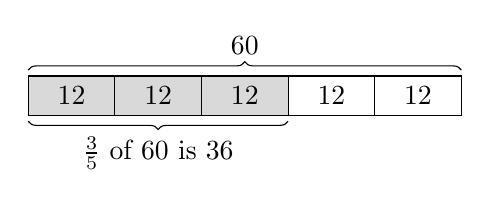
\begin{tikzpicture}[x=11mm,y=5mm]
  \fill[black!15] (0,0) rectangle (3,1);
  \foreach \i in {0,...,4}{\draw (\i,0) rectangle ++(1,1); \node at (\i+0.5,0.5) {12};}
  \draw[decorate,decoration={brace,amplitude=3pt}] (0,1.15) -- (5,1.15) node[midway,above=2pt] {60};
  \draw[decorate,decoration={brace,amplitude=3pt,mirror}] (0,-0.15) -- (3,-0.15) node[midway,below=2pt] {$\frac35$ of 60 is 36};
\end{tikzpicture}

\wq{18} (a) $64\div8=8$, $8\times3=24$\qquad (b) Calculator: $7\div9\times504=392$

\wq{19} $840\div7=120$, and $120\times3=360$ pupils have school dinners, so $840-360=480$ do not.

% ----------------------------------------------------------------
\ptitle{Percentages of amounts}{Per cent means `out of 100'; `of' means multiply by.}

\wq{20} (a) 10\% of $140=14$, 5\% $=7$, so 35\% $=14+14+14+7=49$

(b) 50\% of $64=32$, 25\% $=16$, so 12.5\% $=8$ (halving each time)

\wq{21} (a) $0.23\times85=19.55$\qquad (b) $0.045\times2400=108$, so £108

% ----------------------------------------------------------------
\ptitle{Percentage change}{Change over original, times 100.}

\wq{22} (a) Change $=62-50=12$: $\dfrac{12}{50}\times100=24\%$ increase

(b) Change $=80-68=12$: $\dfrac{12}{80}\times100=15\%$ decrease

\wq{23} Change $=12\,000-9000=3000$: $\dfrac{3000}{12\,000}\times100=25\%$ decrease

% ----------------------------------------------------------------
\ptitle{Simple interest}{Same interest every year: find one year, multiply by years.}

\wq{24} 2\% of £500 $=$ £10 interest every year.

{\renewcommand{\arraystretch}{1.5}%
\begin{tabular}{|l|c|c|c|c|c|}\hline
Year & 0 & 1 & 2 & 3 & 4\\\hline
Balance (£) & 500 & 510 & 520 & 530 & 540\\\hline
\end{tabular}}

\wq{25} 5\% of £800 $=$ £40 a year. Amy needs $1000-800=$ £200 of interest, and $200\div40=5$, so it takes 5 years.

% ----------------------------------------------------------------
\ptitle{Calculating with mixed numbers and negatives}{Mixed $\to$ improper first. Dividing? Keep, change, flip. (KFC)}

\wq{26} (a) $1\frac23+2\frac14=\dfrac53+\dfrac94=\dfrac{20}{12}+\dfrac{27}{12}=\dfrac{47}{12}=3\dfrac{11}{12}$

(b) $4\frac15-1\frac12=\dfrac{21}5-\dfrac32=\dfrac{42}{10}-\dfrac{15}{10}=\dfrac{27}{10}=2\dfrac7{10}$

(c) $1\frac12\times2\frac23=\dfrac32\times\dfrac83=\dfrac{24}6=4$

\wq{27} (a) $3\frac34\div1\frac14=\dfrac{15}4\div\dfrac54=\dfrac{15}4\times\dfrac45=\dfrac{60}{20}=3$

(b) $-\dfrac23\times\dfrac9{10}=-\dfrac{18}{30}=-\dfrac35$

(c) $-1\frac14\div\left(-\dfrac58\right)=-\dfrac54\times\left(-\dfrac85\right)=\dfrac{40}{20}=2$\quad (negative $\times$ negative $=$ positive)

% ----------------------------------------------------------------
\ptitle{Word problems with mixed numbers}{Find the numbers, pick the operation, include units.}

\wq{28} Cut off: subtract.
\[ 5\tfrac14-2\tfrac23=\frac{21}4-\frac83=\frac{63}{12}-\frac{32}{12}=\frac{31}{12}=2\tfrac7{12}\text{ m} \]

\wq{29} How many fit into: divide.
\[ 2\tfrac34\div\tfrac13=\frac{11}4\times\frac31=\frac{33}4=8\tfrac14 \]
Only full glasses count, so 8 glasses.

\wq{30} Area $=$ length $\times$ width
\[ 6\tfrac12\times3\tfrac13=\frac{13}2\times\frac{10}3=\frac{130}6=\frac{65}3=21\tfrac23\text{ m}^2 \]

% ----------------------------------------------------------------
\ptitle{Recurring decimals to fractions}{Line up the repeats, then subtract them away. Solve algebra.}

\wq{31}
\[ \begin{array}{r@{\;}r@{\;=\;}r@{}l}
  \text{Let} & n & 0 & .444\ldots\\
             & 10n & 4 & .444\ldots\\
  \text{subtract:} & 9n & 4 &
\end{array}\qquad n=\frac49 \]

\wq{32} (a) Let $n=0.3636\ldots$ Two digits repeat, so $\times100$:
\[ \begin{array}{r@{\;}r@{\;=\;}r@{}l}
             & 100n & 36 & .3636\ldots\\
             & n & 0 & .3636\ldots\\
  \text{subtract:} & 99n & 36 &
\end{array}\qquad n=\frac{36}{99}=\frac4{11} \]
(b) Let $n=0.8333\ldots$ The 8 does not repeat, so use $100n$ and $10n$ to line up the repeats:
\[ \begin{array}{r@{\;}r@{\;=\;}r@{}l}
             & 100n & 83 & .333\ldots\\
             & 10n & 8 & .333\ldots\\
  \text{subtract:} & 90n & 75 &
\end{array}\qquad n=\frac{75}{90}=\frac56 \]

% ----------------------------------------------------------------
\ptitle{Percentage increase and decrease with multipliers}{100\% plus or minus the change, then $\div100$.}

\wq{33} (a) $100\%+8\%=108\%\to1.08$\qquad (b) $100\%-30\%=70\%\to0.7$\qquad (c) $102.5\%\to1.025$

\wq{34} (a) Up 35\% $\to\times1.35$: $64\times1.35=86.4$, so £86.40

(b) Down 12\% $\to\times0.88$: $1250\times0.88=1100$

% ----------------------------------------------------------------
\ptitle{Finding the original amount}{Going backwards? Divide by the multiplier!}

\wq{35} 30\% off $\to\times0.7$:\quad $0.7\times\text{original}=56\to\text{original}=56\div0.7=$ £80

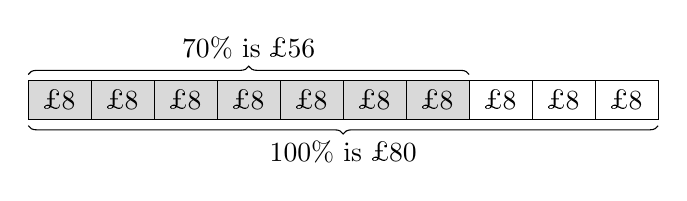
\begin{tikzpicture}[x=8mm,y=5mm]
  \fill[black!15] (0,0) rectangle (7,1);
  \foreach \i in {0,...,9}{\draw (\i,0) rectangle ++(1,1); \node at (\i+0.5,0.5) {£8};}
  \draw[decorate,decoration={brace,amplitude=3pt}] (0,1.15) -- (7,1.15) node[midway,above=2pt] {70\% is £56};
  \draw[decorate,decoration={brace,amplitude=3pt,mirror}] (0,-0.15) -- (10,-0.15) node[midway,below=2pt] {100\% is £80};
\end{tikzpicture}

Check with the bar: 70\% is £56, so 10\% is £8 and 100\% is £80.

\wq{36} Up 10\% $\to\times1.1$:\quad original $=77\div1.1=$ £70

\wq{37} Up 20\% $\to\times1.2$:\quad original $=54\div1.2=$ £45

% ----------------------------------------------------------------
\par\addvspace{10pt}
\noindent\rule{\linewidth}{0.8pt}\par\nobreak\vspace{1pt}
\noindent{\large\bfseries Problem solving}\par\nobreak\vspace{1pt}
\noindent\rule{\linewidth}{0.4pt}\par\nobreak\vspace{4pt}

\wq{38} Shop A: $\frac13$ of $90=30$, so the coat costs £60.

Shop B: $90\times0.7=63$, then $63\times0.95=59.85$, so the coat costs £59.85.

Shop B is cheaper, by $60-59.85=$ £0.15, which is 15p.

\wq{39} Kim has worked forwards from £280, but the 30\% was taken off the original price, not off £280. Going backwards, we divide by the multiplier: 30\% off $\to\times0.7$, so
\[ \text{original}=280\div0.7=\text{£}400 \]
Check: 30\% of £400 is £120, and $400-120=280$. Kim's £364 does not work: 30\% off £364 is £254.80.

\wq{40} $\frac35=0.6$ and $\frac7{10}=0.7$, so any fraction whose decimal is between 0.6 and 0.7 will do. For example
\[ \frac{13}{20}=0.65\qquad \frac{31}{50}=0.62\qquad \frac23=0.666\ldots \]
Another way: with denominator 40, $\frac35=\frac{24}{40}$ and $\frac7{10}=\frac{28}{40}$, so $\frac{25}{40}$, $\frac{26}{40}$ and $\frac{27}{40}$ are all in between.

\end{document}
